% !TeX root = ../thuthesis-example.tex

\chapter{计算图中间表示与高级语言代码的相互转换}
\label{chp:eng}

\section{实现动机}

NNSmith 中没有显式地对所生成计算图进行表示,而是用 Python 内置列表存储计算图上的各个算子,用字典存储各个张量,在执行计算图时采用循环语句依次执行列表中的算子。然而,这种用一套通用代码运行所有模型的实现方式存在以下两个问题:
\begin{enumerate}
    \item \textbf{干扰深度学习编译器的正常工作。} 对于高级编程语言描述的深度学习模型,深度学习编译器需先对其进行解析,将其行为建模为计算图,然后对计算图做优化。但在解析高级语言方面,深度学习编译器往往不能支持高级语言的全部语法,而只为其中常用的子集提供支持。然而, NNSmith 中的通用模型执行逻辑较为复杂,除了对张量值进行简单的前向传播以外,还实现了提升数值合法性所需的损失值计算与梯度维护等逻辑,其中引入了较多的自定义类与方法,这对深度学习编译器的解析工作不友好。
    如近期新发布的 PyTorch 2.0 \cite{pt2_release} 中的编译接口 \texttt{torch.compile} ,在对 NNSmith 中的模型运行过程进行编译时,就会因不支持的 Python 语法报错而编译失败,因此 NNSmith 无法对这一新推出的编译框架进行测试。
    \item \textbf{给漏洞检查与汇报等人工后处理带来困难。} 上述 NNSmith 的模型执行过程在 Python 代码的实现上有百余层,并且由于对所有模型的执行通用,无法直观地看出计算图的结构与执行过程。因此,对每个 NNSmith 找到的潜在漏洞,我们不能让深度学习框架的开发者运行一整套复杂的 NNSmith 代码来复现,否则会带来较大负担。相反,我们需要对照 NNSmith 输出的包含算子列表与对应输入输出张量的元信息,手工编写可复现漏洞的、最小化的、可独立运行的代码,将其作为漏洞报告的核心部分提交至开发者团队。然而,人工对每个漏洞依次进行编写最小可复现代码、验证其仍能够触发漏洞、以及收集运行日志的一系列操作较为繁琐,会花费较长时间。
\end{enumerate}
因此,我们需要实现从所生成的计算图,到高级语言描述的、最小可复现代码的转换过程,以清晰直观地呈现可触发漏洞的代码逻辑,并减轻漏洞复现与汇报的人工负担。

此外, NNSmith 从零开始构建计算图,没有利用任何真实世界代码;本文在计算图生成时引入了来自真实世界代码的具体算子,在单个算子层面利用了已存在的代码来构造测例。而未来可以探索的方向之一是在多算子层面利用已经存在的代码,来源包括已被修复漏洞的触发代码中的片段、开源项目中的模型片段、以及 ChatGPT\cite{chatgpt}等大语言模型生成的代码片段等,在这些片段的基础上进行编译,以构造测例。而为了利用已存在代码片段并进行变异操作,需要实现从 Python 代码片段到 NNSmith 中计算图表示的转换过程。

综上,我们需要实现计算图表示与 Python 代码的相互转换。由于这一功能主要对测试 PyTorch 2.0 中的编译器有较大帮助、 PyTorch 框架中的配套支持较为完善、并且 PyTorch 开发团队对我们所汇报漏洞的响应较为积极,因此我们暂时只为 PyTorch 框架实现这一功能。

\section{实现方法}

NNSmith 的开发者近期实现了一种供模糊测试所用的计算图中间表示 GraphIR ,以将模型的生成与变异逻辑与下层具体的深度学习框架解耦。而 PyTorch 的 fx 模块\cite{torch_fx}亦为编译过程所需的计算图提供了一种中间表示,并实现了这种中间表示与 Python 可执行代码之间的相互转换。因此,如图 \ref{fig:convert} 所示,我们只需实现 NNSmith GraphIR 与 PyTorch fx 模块之间的相互转换,便可以实现模糊测试框架中计算图的中间表示与 Python 代码的相互转换。

\begin{figure}
    \centering
    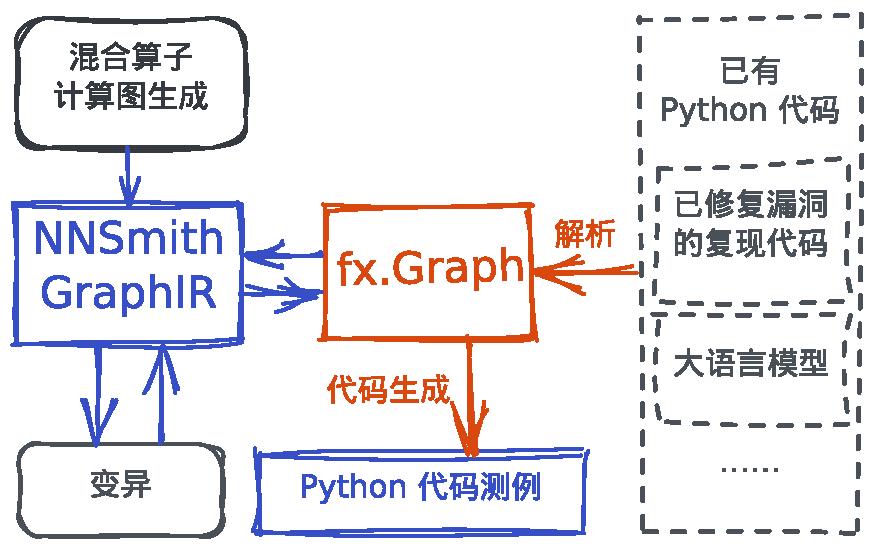
\includegraphics[width=.8\linewidth]{figures/convert.pdf}
    \caption{中间表示与代码间的转换}
    \label{fig:convert}
\end{figure}

\subsection{NNSmith 计算图中间表示简介}

在 NNSmith GraphIR 中,每个计算图由如图 \ref{fig:instir} 所示的若干 InstIR 结构组成。 InstIR 结构包含两部分,分别是输出张量的变量名,和 InstExpr 结构。后者又包括两部分,分别是除了张量输入的其它参数输入都已固定的可调用接口,即算子,与输入张量变量名。之所以将张量输入与其余参数输入分开,是因为在计算图中,我们主要关心的数据流是张量。

\begin{figure}
    \centering
    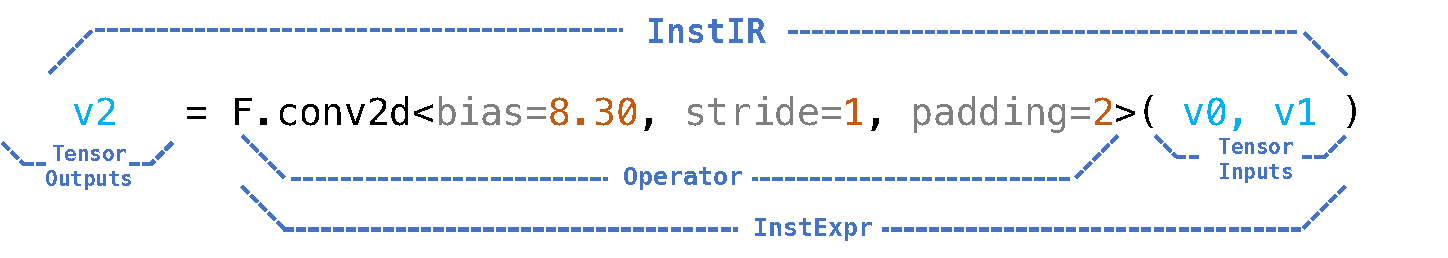
\includegraphics[width=1.\linewidth]{figures/instir.pdf}
    \caption{InstIR 结构示意}
    \label{fig:instir}
\end{figure}

\subsection{PyTorch 计算图中间表示简介}
\label{fxir}

PyTorch 中的 fx 模块提供了计算图的中间表示。如对于代码 \texttt{v = F.conv2d(x, kernel, 8.30, stride=1, padding=2)} , fx 模块可以将其转化为一个中间表示节点,节点上存有以下字段:

\begin{itemize}
    \item \texttt{opcode: call\_function} :意指此节点的操作类型是调用一个函数。
    \item \texttt{name: conv2d} :意为此节点的输出在中间表示中被记为 \texttt{conv2d} 。
    \item \texttt{target: <built-in method conv2d of type object at 0x7f68814c5400>} :存储了此节点所调用的函数的引用。
    \item \texttt{args: (arg0, arg1, tensor)} :列举了调用 \texttt{target} 时的“位置型参数”(positional arguments)。
    \item \texttt{kwargs: {'stride': 1, 'padding': 2}} :列举了调用 \texttt{target} 时的“关键词型参数”(keyword arguments)。
\end{itemize}

可见, PyTorch fx 模块对于接口调用的表示没有以张量数据为中心,只区分了“位置型参数”与“关键词型参数”,而将张量输入与其余输入混合在一起。但是,无论是生成计算图还是对现有计算图做变异,主要考虑的是张量数据的合法匹配问题。因此,相比之下, NNSmith 的计算图中间表示更适用于在模糊测试的背景下操作计算图的场景,为其实现与深度学习框架中的计算图表示之间的转换是值得的。

\subsection{具体实现}

对于给定的进行 PyTorch 张量运算的 Python 代码,我们首先利用 PyTorch 2.0 中推出的 TorchDynamo 模块将其转换为 fx 模块中的计算图。然后,我们遍历已经拓扑排序好的计算图中的各个节点,解析 \ref{fxir} 中介绍的节点上存储的各个字段。我们递归地遍历 \texttt{args} 和 \texttt{kwargs} 两个字段中的每个参数,将张量参数与其余参数分开,从而如图 \ref{fig:instir} 所示,构造其余参数固定的算子,以及输入张量列表,进而形成 \texttt{InstExpr} 结构;然后我们在计算图中新建一个 \texttt{InstIR} 实例,并获取其自动为每个输出张量分配的变量名。由于 fx 模块中的计算图中间表示对变量的命名规则与 NNSmith 不同,因而此处需要根据输出张量在两种中间表示中的不同名称全程维护映射关系,以在后续节点的转化中将 fx 中的输入张量名映射为 NNSmith GraphIR 中的变量名。值得注意的是, fx 模块中间表示中的每个节点均只输出一个变量,对于 \texttt{torch.split} 等输出多变量的节点,会先存为元组,然后通过额外的调用 \texttt{getitem} 方法的节点来获取其中的某个变量。而 NNSmith GraphIR 中表示一个张量操作的 \texttt{InstIR} 结构支持多变量输出,因此我们将做特殊处理,将额外的 \texttt{getitem} 节点压缩至输出多变量的节点中,从而简化计算图的表示,便于对其进行变异。

从 NNSmith GraphIR 向 fx 模块中间表示的转换是上述过程的逆过程,其原理相同且实现类似,因而在此不做赘述。

\section{实现效果}

代码 \ref{listing:nnsmith_forward} 描述了 NNSmith 中前向传播任意模型的实现(删去了为提升数值合法性的逻辑);代码 \ref{listing:gencode} 描述了基于上述 NNSmith GraphIR 到 fx 模块中间表示的转换,再结合 fx 模块从中间表示生成代码的功能,综合出的可独立运行并可复现漏洞的程序。
其中,模型定义中的 \texttt{forward} 函数(第 \ref{listing:gencode:forward} 行)由 fx 模块生成,代码其余部分基于我们定义的模板生成,包括模型定义(第 \ref{listing:gencode:modelinit} 行)、模型权重初始化(第 \ref{listing:gencode:winit} 行)、输入构造(第 \ref{listing:gencode:inputinit} 行)、模型编译(第 \ref{listing:gencode:modelcomp} 行)、解释模式执行(第 \ref{listing:gencode:eagerrun} 行)、编译模式执行(第 \ref{listing:gencode:comprun} 行)与差分测试(第 \ref{listing:gencode:diff} 行)。
可以看出,代码 \ref{listing:gencode} 清晰地描述了具体模型的结构,并能够执行差分测试寻找漏洞,相比前者便于独立运行、修改与调试,可以直接作为漏洞报告的一部分提交至开发者团队。

\begin{listing}[]
    \caption{简化版 NNSmith 前向传播实现}
    \label{listing:nnsmith_forward}
\begin{minted}[
    fontsize=\small,
    linenos, mathescape, escapeinside=||,
    % texcomments,
    frame=lines,
    framesep=1.5mm,    
]{python}
def forward(self, *args, **kwargs):
    tensor_map: Dict[str, torch.Tensor] = {}

    if len(args) == len(self.input_map):
        for i, key in enumerate(self.ir.input_var()):
            tensor_map[key] = args[i]
    elif len(kwargs) == len(self.input_map):
        for ir_key in self.input_map:
            tensor_map[ir_key] = kwargs[ir_key]
    else:
        raise ValueError("Use either args or kwargs only")

    for stmt_idx, instruction in enumerate(self.instructions):
        inst, inps, outs, op = instruction
        input_tensors = [tensor_map[idx] for idx in inps]

        # REAL FORWARD.
        output_tensors = inst(*input_tensors)
        if isinstance(output_tensors, torch.Tensor):
            output_tensors = [output_tensors]
        if isinstance(output_tensors, tuple):
            output_tensors = list(output_tensors)
        output_tensors = output_tensors[: len(op.output_like)]

        for i, out_key in enumerate(outs):
            # put values back to tensor_map.
            tensor_map[out_key] = output_tensors[i]
            
    return tuple(tensor_map[key] for key in self.output_map)
\end{minted}
\end{listing}

\begin{listing}[]
    \caption{从中间表示生成的测例代码}
    \label{listing:gencode}
\begin{minted}[
    fontsize=\small,
    linenos, mathescape, escapeinside=||,
    % texcomments,
    frame=lines,
    framesep=1.5mm,    
]{python}
import numpy as np
import torch
import pickle

# Model definition
class M(torch.nn.Module):
    def __init__(self): |\label{listing:gencode:modelinit}|
        super().__init__()
        self.conv = torch.nn.Conv2d(
            3, 3, kernel_size=(3, 3), stride=(1, 1))
        self.bn = torch.nn.BatchNorm2d(
            3, eps=1e-05, momentum=0.1,
            affine=True, track_running_stats=True)
        self.linear = torch.nn.Linear(
            in_features=62, out_features=3, bias=True)

    def forward(self, x): |\label{listing:gencode:forward}|
        conv = self.conv(x);  x = None
        bn = self.bn(conv);  conv = None
        linear = self.linear(bn);  bn = None
        return linear

m = M()

|\label{listing:gencode:winit}|# Initialize weight
# None

|\label{listing:gencode:inputinit}|# Initialize input
inp = [np.zeros([1, 3, 64, 64], dtype='float32')]

|\label{listing:gencode:modelcomp}|# Compile the model
opt = torch.compile(m, fullgraph=True, backend='inductor')

|\label{listing:gencode:eagerrun}|# Eager run
m_out = m(*[torch.from_numpy(v).to('cpu') for v in inp])
m_out = [v.cpu().detach() for v in m_out] # torch2numpy
m_out = [v.resolve_conj().numpy() if v.is_conj()
    else v.numpy() for v in m_out] # torch2numpy

|\label{listing:gencode:comprun}|# Compiled run
opt_out = opt(*[torch.from_numpy(v).to('cpu') for v in inp])
opt_out = [v.cpu().detach() for v in opt_out] # torch2numpy
opt_out = [v.resolve_conj().numpy() if v.is_conj()
    else v.numpy() for v in opt_out] # torch2numpy

|\label{listing:gencode:diff}|# Differential testing
for i, (l, r) in enumerate(zip(m_out, opt_out)):
    np.testing.assert_allclose(l, r, rtol=1e-2, atol=1e-3,
        err_msg=f"Result mismatch @ index {i}")
\end{minted}
\end{listing}

\iffalse
\chapter{引用文献的标注}

模板支持 BibTeX 和 BibLaTeX 两种方式处理参考文献。
下文主要介绍 BibTeX 配合 \pkg{natbib} 宏包的主要使用方法。


\section{顺序编码制}

在顺序编码制下,默认的 \cs{cite} 命令同 \cs{citep} 一样,序号置于方括号中,
引文页码会放在括号外。
统一处引用的连续序号会自动用短横线连接。

\thusetup{
  cite-style = super,
}
\begin{tabular}{l@{\quad$\Rightarrow$\quad}l}
  \verb|\cite{zhangkun1994}|               & \cite{zhangkun1994}               \\
  \verb|\citet{zhangkun1994}|              & \citet{zhangkun1994}              \\
  \verb|\citep{zhangkun1994}|              & \citep{zhangkun1994}              \\
  \verb|\cite[42]{zhangkun1994}|           & \cite[42]{zhangkun1994}           \\
  \verb|\cite{zhangkun1994,zhukezhen1973}| & \cite{zhangkun1994,zhukezhen1973} \\
\end{tabular}


也可以取消上标格式,将数字序号作为文字的一部分。
建议全文统一使用相同的格式。

\thusetup{
  cite-style = inline,
}
\begin{tabular}{l@{\quad$\Rightarrow$\quad}l}
  \verb|\cite{zhangkun1994}|               & \cite{zhangkun1994}               \\
  \verb|\citet{zhangkun1994}|              & \citet{zhangkun1994}              \\
  \verb|\citep{zhangkun1994}|              & \citep{zhangkun1994}              \\
  \verb|\cite[42]{zhangkun1994}|           & \cite[42]{zhangkun1994}           \\
  \verb|\cite{zhangkun1994,zhukezhen1973}| & \cite{zhangkun1994,zhukezhen1973} \\
\end{tabular}



\section{著者-出版年制}

著者-出版年制下的 \cs{cite} 跟 \cs{citet} 一样。

\thusetup{
  cite-style = author-year,
}
\begin{tabular}{l@{\space$\Rightarrow$\space}l}
  \verb|\cite{zhangkun1994}|                & \cite{zhangkun1994}                \\
  \verb|\citet{zhangkun1994}|               & \citet{zhangkun1994}               \\
  \verb|\citep{zhangkun1994}|               & \citep{zhangkun1994}               \\
  \verb|\cite[42]{zhangkun1994}|            & \cite[42]{zhangkun1994}            \\
  \verb|\citep{zhangkun1994,zhukezhen1973}| & \citep{zhangkun1994,zhukezhen1973} \\
\end{tabular}

\vskip 2ex
\thusetup{
  cite-style = super,
}
注意,引文参考文献的每条都要在正文中标注
\cite{zhangkun1994,zhukezhen1973,dupont1974bone,zhengkaiqing1987,%
  jiangxizhou1980,jianduju1994,merkt1995rotational,mellinger1996laser,%
  bixon1996dynamics,mahui1995,carlson1981two,taylor1983scanning,%
  taylor1981study,shimizu1983laser,atkinson1982experimental,%
  kusch1975perturbations,guangxi1993,huosini1989guwu,wangfuzhi1865songlun,%
  zhaoyaodong1998xinshidai,biaozhunhua2002tushu,chubanzhuanye2004,%
  who1970factors,peebles2001probability,baishunong1998zhiwu,%
  weinstein1974pathogenic,hanjiren1985lun,dizhi1936dizhi,%
  tushuguan1957tushuguanxue,aaas1883science,fugang2000fengsha,%
  xiaoyu2001chubanye,oclc2000about,scitor2000project%
}。
\fi
